For simplicity, we begin with an evaluation of the signal over A/B outright
winner market pairs for tennis ATP matches between 2017/08/01 and 2017/09/30
(amounts to a total of 347 events where 220 are actually traded). Though the
existence of cointegration within this pairing is unclear, there is a much
stronger guarantee of liquidity which makes for less sparse backtest results.

The following assumptions are made about the environment
\begin{enumerate}
    \item Zero in-play delay.
    \item Immediate execution at either the mid-price or top of the book ---
        this also implies that we do not consider prevalent effects such as
        adverse selection.
    \item Perfect connection such that we experience zero latency and no loss of
        messages in transit to the exchange.
    \item We do not consider path dependency (perhaps due to randomness) or any
        of the complexities associated with cashing out, amounting to an
        assumption of infinite liquidity.
\end{enumerate}

\subsection{Mid-price execution}
Here we assume that the agent is executed favourably at the mid-prices of the
two legs. Thus, the strategy effectively tracks the spread series, taking a
long, short or neutral position based on the cointegration signal.

A few key observations:
\begin{enumerate}
    \item For the short holding period we consider here (until the next time
        step) short lookback windows are favourable
        (Fig.~\ref{fig:mp_nodelay:pnl}).
    \item The sub-sampling rate appears to have a considerable effect on the
        performance, though this relationship is not the same of all lookback
        windows. Crucially, for the 200 period window, larger values for the
        sampling-rate (sampling less) have lower associated variance.
    \item The proportion of wins to losses behaves in the opposite way, where
        larger values of the sub-sampling rate have increased variance and a
        greater proportion of outlier cases (Fig.~\ref{fig:mp_nodelay:propwl}).
    \item The consistency ratio appears to be best for larger lookback windows
        and low sampling rates.
\end{enumerate}

\begin{figure}[H]
    \centering
    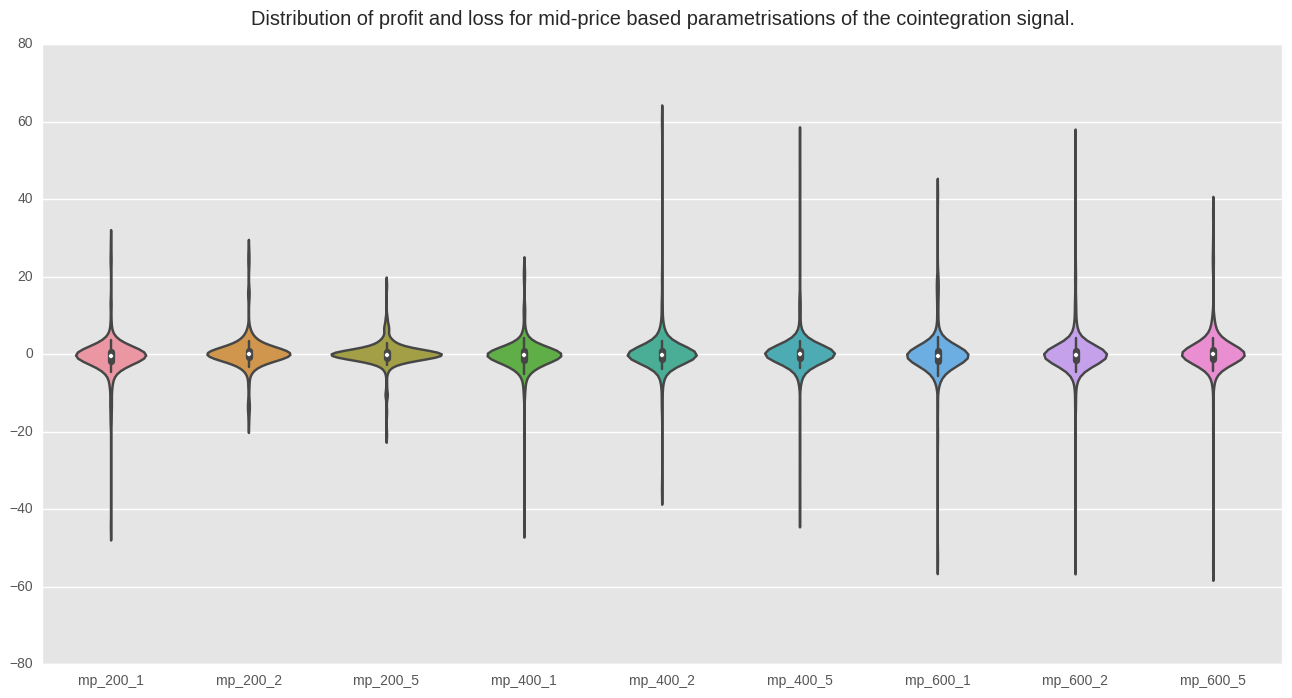
\includegraphics[width=\figwidth]{img/mp_nodelay.png}

    \caption{}\label{fig:mp_nodelay:pnl}
\end{figure}

\begin{figure}[H]
    \centering
    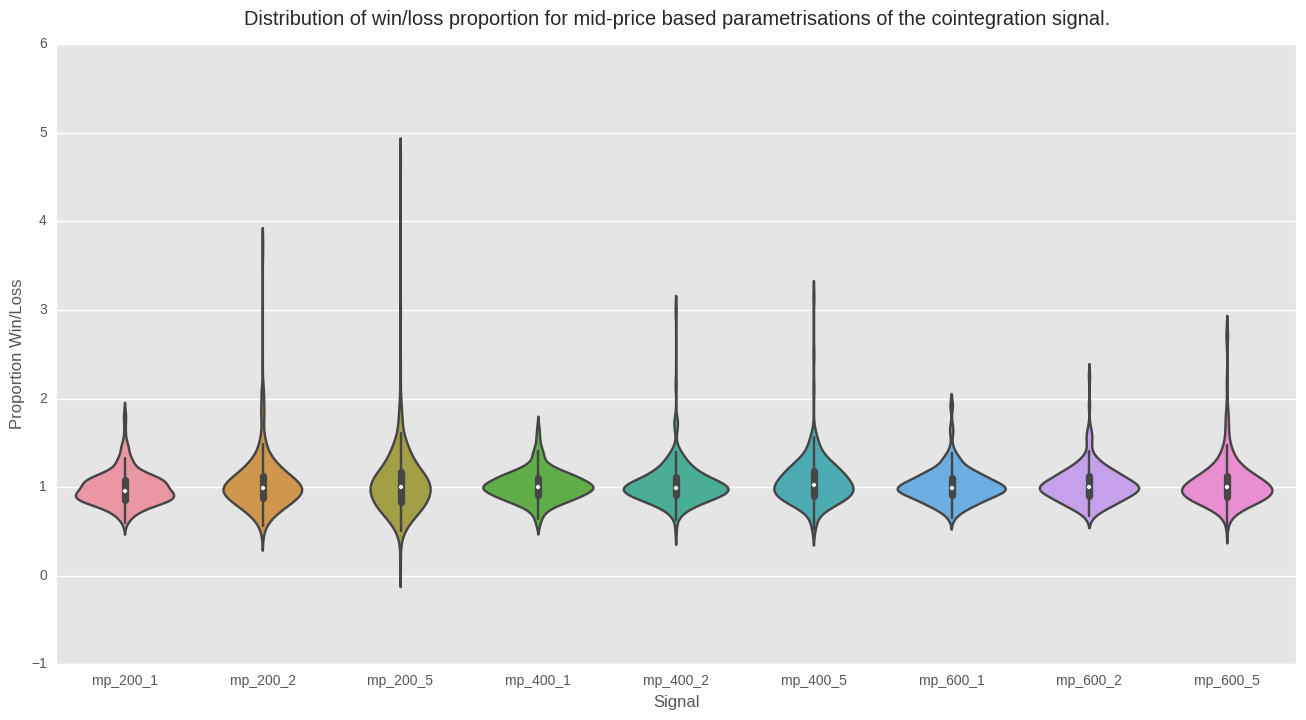
\includegraphics[width=\figwidth]{img/mp_nodelay_propwl.png}

    \caption{}\label{fig:mp_nodelay:propwl}
\end{figure}

\begin{figure}[H]
    \centering
    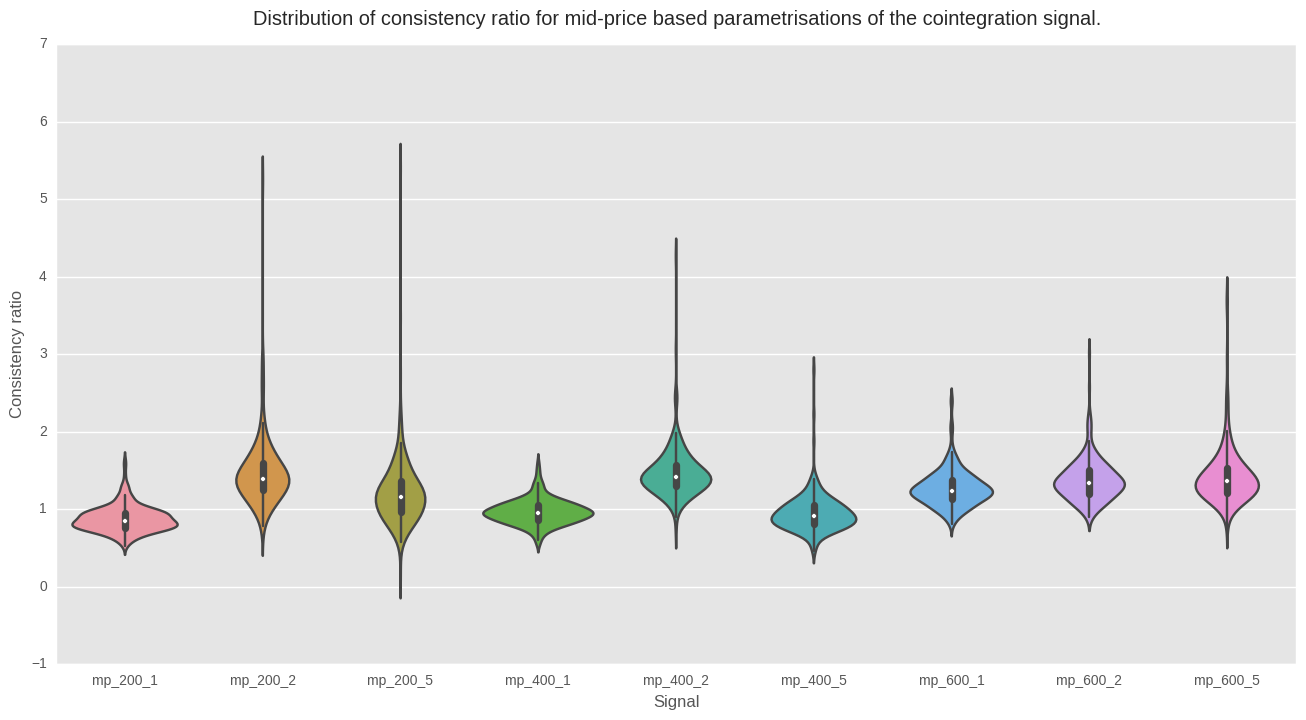
\includegraphics[width=\figwidth]{img/mp_nodelay_cr.png}

    \caption{}\label{fig:mp_nodelay:cr}
\end{figure}

\subsection{Spread crossing execution}
Here we assume that the agent always crosses the spread, walking the book in
each of the two legs.

A few observations:
\begin{enumerate}
    \item The strategy performs very poorly when crossing the spread on every
        trade opportunity. This is likely due to the fact that the holding time
        is very short, so the cost of entry/exit are applied very frequently.
    \item Win/loss proportion is also very poor. Further the consistency ratio
        shows that the strategy was never profitable on a step-by-step basis.
        Again, we need longer and/or more informed holding times.
\end{enumerate}

\begin{figure}[H]
    \centering
    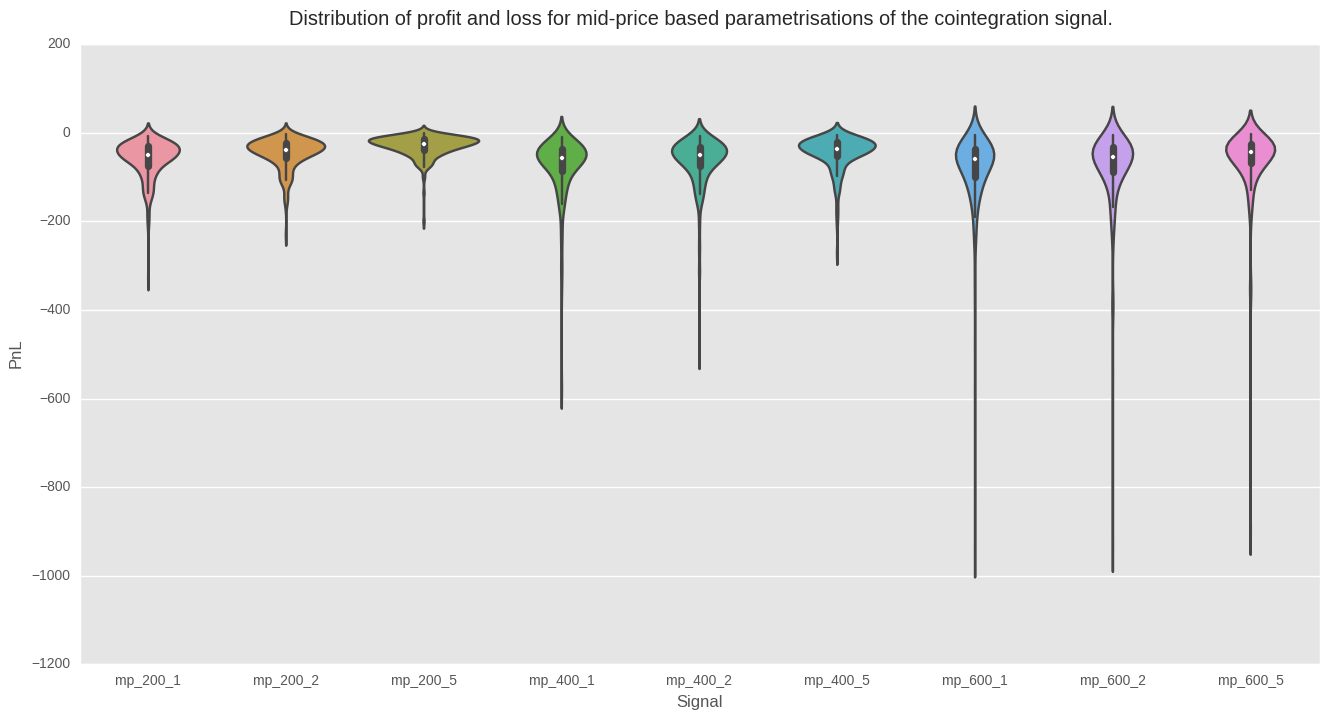
\includegraphics[width=\figwidth]{img/sp_nodelay.png}

    \caption{}\label{fig:sp_nodelay:pnl}
\end{figure}

\begin{figure}[H]
    \centering
    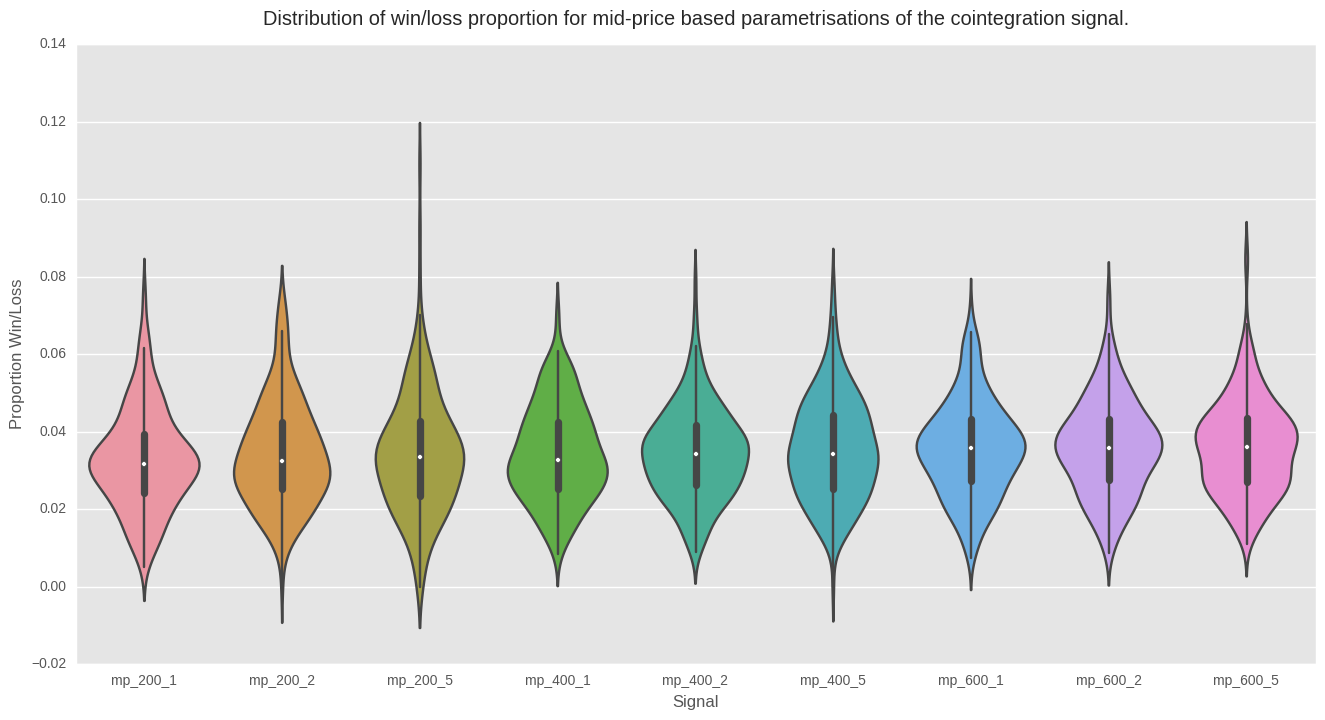
\includegraphics[width=\figwidth]{img/sp_nodelay_propwl.png}

    \caption{}\label{fig:sp_nodelay:propwl}
\end{figure}

\begin{figure}[H]
    \centering
    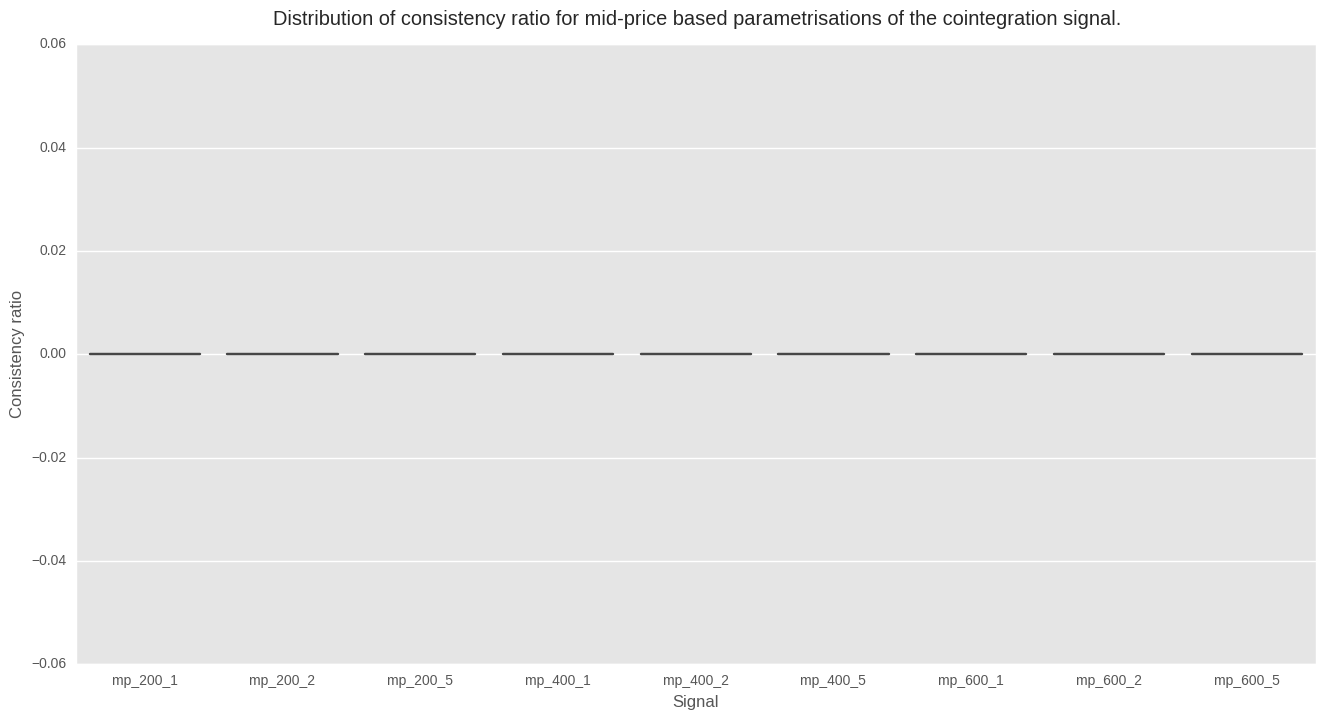
\includegraphics[width=\figwidth]{img/sp_nodelay_cr.png}

    \caption{}\label{fig:sp_nodelay:cr}
\end{figure}
